\section{Experiments and applications}
\label{sec:uses}
\subsection{Experimental setting}

\paragraph{Implementation details.}
The simulations have been conducted in Python, including for the \palm algorithm.
Running times are measured on computer grid with 3.8GHz-CPUs (2.5GHz in Figure~\ref{fig:time_csr}).
Fast operators $\rmV$ based on sparse matrices $\rmS_q$ are implemented with \texttt{csr\_matrix} objects from the \texttt{scipy.linalg} package. 
While more efficient implementations may be beneficial for larger deployment, our implementation is sufficient as a proof of concept for assessing the performance of the proposed approach. 
In particular, the running times of fast operators of the form $\prod_{q\in\intint{\nfactors}}{\rmS_q}$ have been measured when applying to random vectors, for several sparsity levels: 
as shown in Figure~\ref{fig:time_csr}, they are significantly faster than dense operators -- implemented as a \texttt{numpy.ndarray} matrix --, especially when the data size is larger than $10^3$.


\begin{figure}[tbh]
\centering
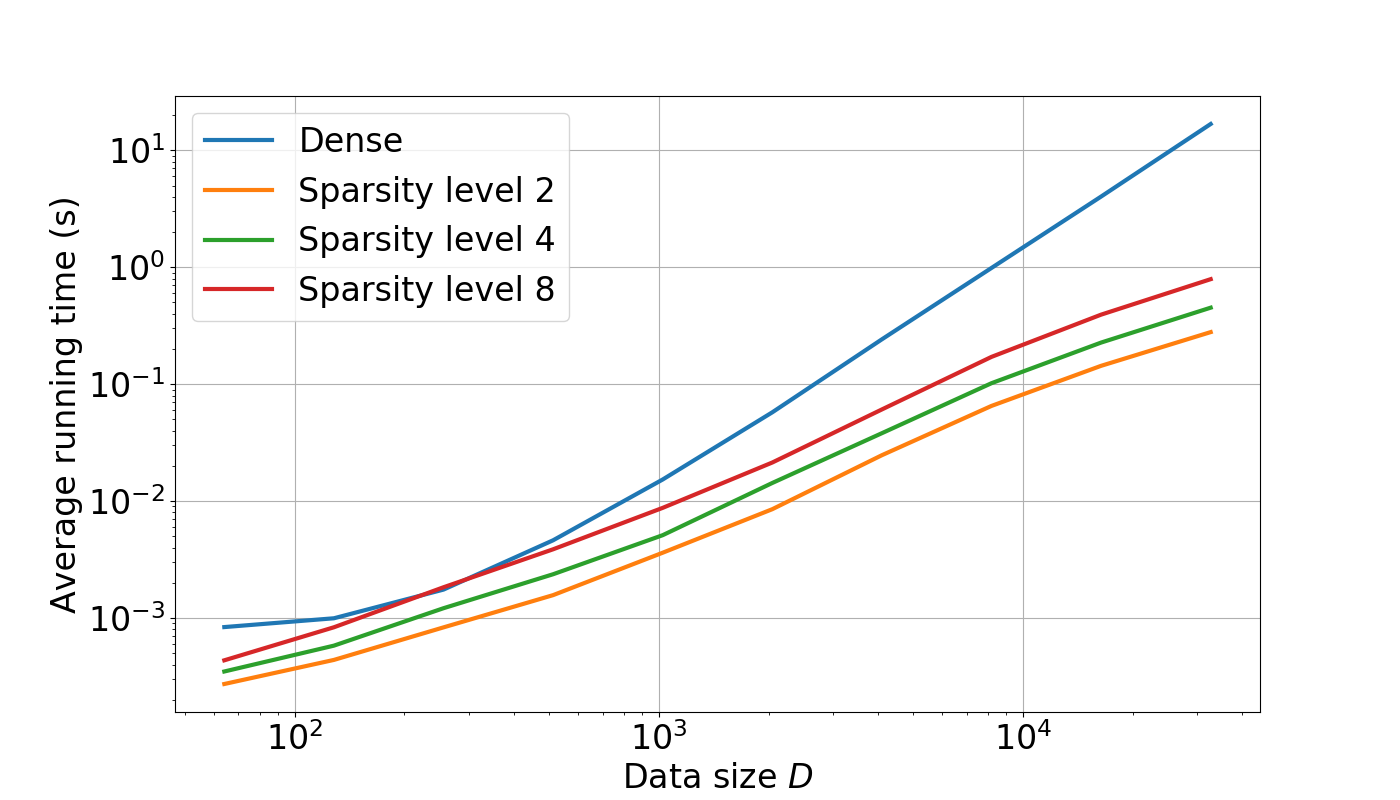
\includegraphics[width=.8\textwidth]{RunningTime4VaryingSparsity.png}
\caption{Running times, averaged over 30 runs, when applying dense or fast $\datadim \times \datadim$ operators to a set of 100 random vectors. The number of factors in fast operators equals $\log_2\left (\datadim\right )$ and the sparsity level denotes the number of non-zero coefficients per row and per column in each factor. \addLG{la figure 1 est très étrange: elle présente une vitesse d'exécution toujours plus rapide pour les opérateurs rapides, peu importe la taille de la matrice. Es-tu sur que cette figure correspond bien à un produit de facteurs sparses? Voir figure \ref{fig:time_csr_fixed_row_size}}\addVE{J'ai fait tourner l'expé (dernière version de \texttt{script\_time\_sparsity.py}) sur le cluster avec un nombre plus importants de runs qu'avant et des dimensions plus importantes. Tu peux regarder une autre figure un peu plus détaillée \texttt{nips\_2019/figures/RunningTime4VaryingSparsity\_with\_area.png} où la zone colorée correspond à la zone de tous les temps mesurés (i.e., entre le min et le max): on voit que pour des petites dimensions, il y a une grosse variance sur le temps de calcul pour les matrices denses. Donc ces résultats ne me semblent pas incompatibles avec les tiens et ceux qu'on avait précédemment; l'essentiel reste à mon sens qu'il faut travailler en grande dimension. À noter que je viens de relancer les expés sur decoda2 car je l'avais fait jusqu'ici sur sensei1 où les CPU sont à 2 ou 2.5GHz.}}
\label{fig:time_csr}
\end{figure}

%\begin{figure}[tbh]
%\centering
%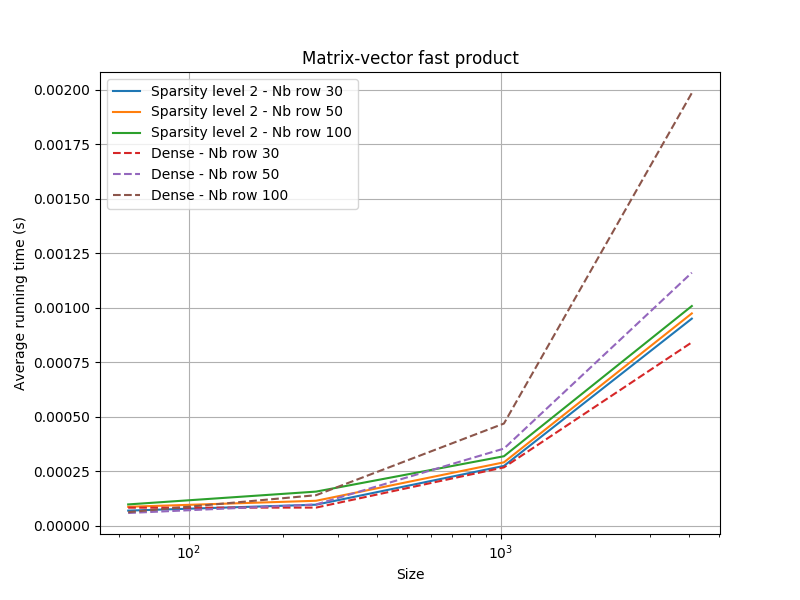
\includegraphics[width=.8\textwidth]{Run_time_sparsity_2.png}
%\caption{Running times, averaged over 30 runs, when applying dense or product of fast operators to a set of 100 random vectors. The number of factors in fast operators equals $\log_2\left (\#~row\right )$ and the sparsity level denotes the number of non-zero coefficients per row and per column in each factor.}
%\label{fig:time_csr_fixed_row_size}
%\end{figure}


\paragraph{Datasets.}
We present results on real-world and toy datasets summarized in Table \ref{table:data}. On the one hand, the real world datasets \texttt{MNIST}~\cite{lecun-mnisthandwrittendigit-2010}, \texttt{Fashion-Mnist}~\cite{Pedregosa2011Scikit} and \texttt{Labeled Faces in the Wild}~\cite{Huang07e.:labeled} (\texttt{LFW}) are used to show --- quantitatively and qualitatively --- the good quality of the obtained centroids when using our method \qkmeans. On the other hand, we use the \texttt{blobs} synthetic dataset from \texttt{sklearn.dataset} to show the speed up offered by our method \qkmeans when the number of clusters and the dimensionality of the data are sufficiently large.
%The code of our method \qkmeans is available on request and will be available online soon. \addLG{je serais d'avis de ne pas dire ça mais soit de dire qu'il est déjà disponible, soit de ne rien dire. Sachant qu'on ne peut pas dire qu'il est déjà disponible en ligne avant le processus de reviewing}


\begin{table*}[!h]
\centering
\begin{tabular}{|c|c|c|c|c|c|}
\hline
\textbf{Dataset} & \textbf{Data dim.} $\datadim$        & \textbf{\# classes} & \textbf{Training set size} $\nexamples$ & \textbf{Test set size} $\nexamples'$ \\ \hline
MNIST                   & 784   & 10        & 60 000    & 10 000               \\ \hline
Fashion-MNIST           & 784   & 10        & 60 000    & 10 000               \\ \hline
LFW                     & 1850  & 2529      & 8866      & N/A               \\ \hline
Blobs (clusters std: 12)   & 2000  & 1000      & 29000      & 1000               \\ \hline
\end{tabular}
\caption{Datasets statistics}
\label{table:data}
\end{table*}


\paragraph{Algorithm settings.} 
The \qkmeans algorithm is used with $Q\eqdef\log_2\left (A\right )$ sparse factors, where  $A=\min\left (\nclusters, \datadim\right )$. 
All factors $\rmS_q$ are with shape $A \times A$ except, depending on the shape of $\rmA$, the leftmost one ($\nclusters\times A$) or the rightmost one ($A\times\datadim$). 
The sparsity constraint of each factor $\rmS_q$ is set in $\mathcal{E}_q$ and is governed by a global parameter denoted as \textit{sparsity level}, which indicates the desired number of non-zero coefficients in each row and in each column of $\rmS_q$. 
Since the projection onto this set of structured-sparsity constraints may be computationally expensive, this projection is relaxed in the implementation of \palm and only guarantees that the number of non-zero coefficients in each row and each column is at least the sparsity level, as in~\cite{LeMagoarou2016Flexible}.
The actual number of non-zero coefficients in the sparse factors is measured at the end of the optimization process and reported in the results.
The sparse factors are updated using the \palm rather than its hierarchical version, since we observed that this was a better choice in terms of computational cost, with satisfying approximation results.
Additional details about \palm are given in Appendix~\ref{sec:app:palm4msa}.
The stopping criterion of \kmeans and \qkmeans consists of a tolerance set to $10^{-6}$ on the relative variation of the objective function and a maximum number of iterations set to 10 for the \texttt{Blobs}dataset and to 20 for others. The same principle governs the stopping criterion of \palm with a tolerance set to $10^{-6}$ and a maximum number of iterations set to 300.

%\subsection{Sparse factors multiplication}
%
%\subsubsection{Sparse factor object}

%\todo[inline]{Parler ici de la configuration de \qkmeans: $Q\eqdef\log_2\left (A\right )$, critère d'arrêt (nombre d'itération, tolérance), ordre des mises à jours, palm4msa plutôt que la version hiérarchique, taille des matrices $\rmS_q$, scaling coefficient, définition de 	$\mathcal{E}_q$.
%}

\subsection{Clustering}

\begin{figure}
\begin{subfigure}[b]{.49\textwidth}
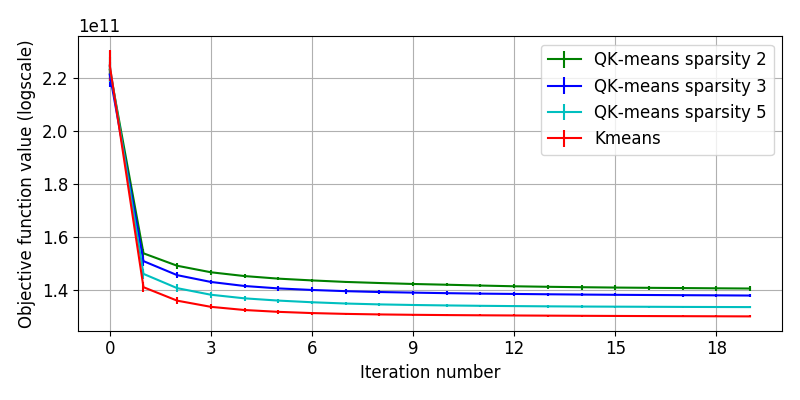
\includegraphics[width=\textwidth]{mnist30_objective.png}
\caption{MNIST, $\nclusters=30$: objective function.}
\label{fig:mnist:objfun}
\end{subfigure}
\begin{subfigure}[b]{.49\textwidth}
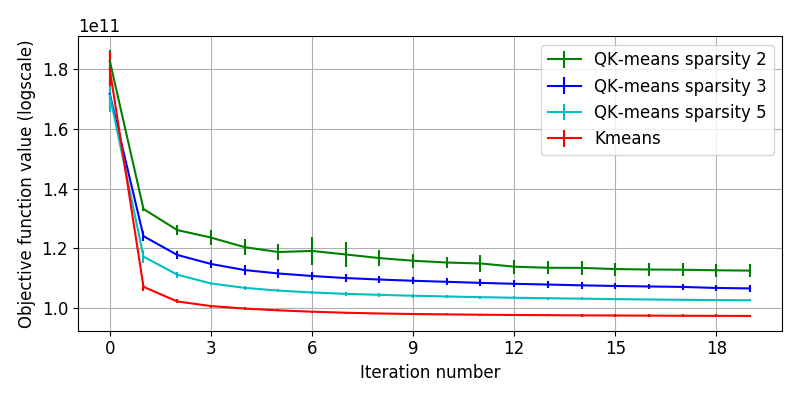
\includegraphics[width=\textwidth]{fashmnist30_objective.png}
\caption{Fashion-MNIST, $\nclusters=30$: objective function.}
\label{fig:fmnist:objfun}
\end{subfigure}
\begin{subfigure}[t]{.49\textwidth}
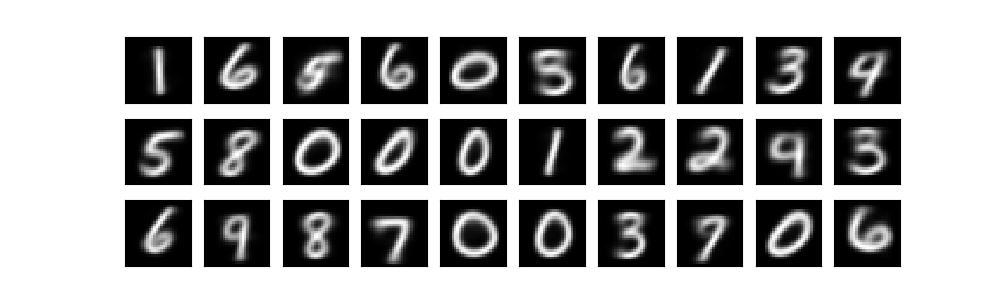
\includegraphics[width=\textwidth]{mnist30_kmeans_centroids.png}
\caption{\kmeans centroids.}
\label{fig:mnist:kmeans:centroids}
\end{subfigure}
\begin{subfigure}[t]{.49\textwidth}
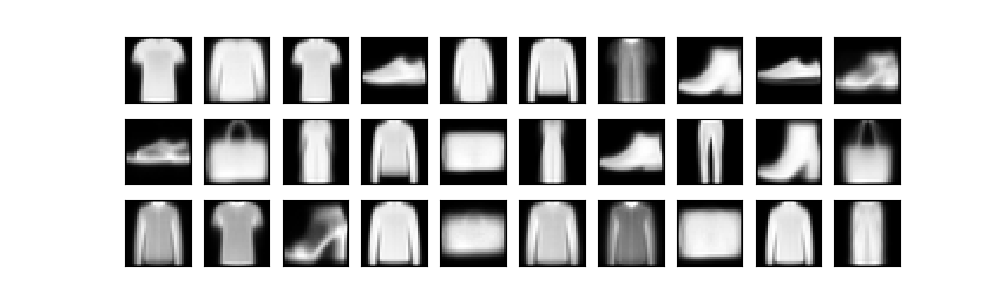
\includegraphics[width=\textwidth]{fashmnist30_kmeans_centroids.png}
\caption{\kmeans centroids.}
\label{fig:fmnist:kmeans:centroids}
\end{subfigure}
\begin{subfigure}[t]{.49\textwidth}
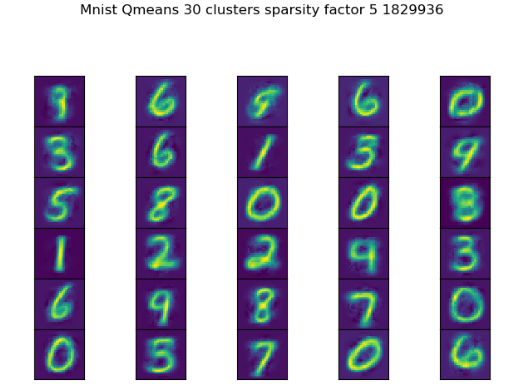
\includegraphics[width=\textwidth]{mnist30_qkmeans_centroids.png}
\caption{\qkmeans centroids.}
\label{fig:mnist:qkmeans:centroids}
\end{subfigure}
\begin{subfigure}[t]{.49\textwidth}
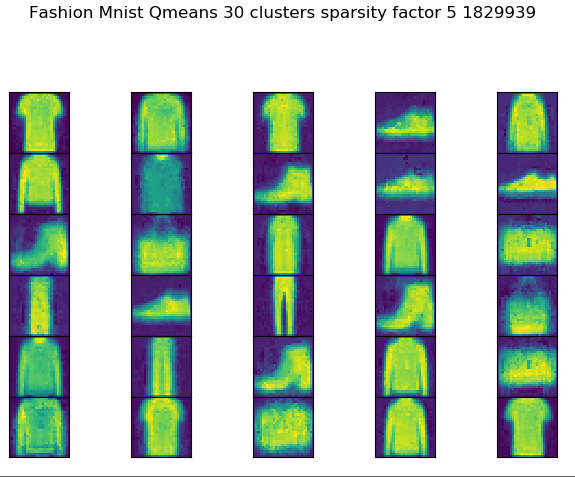
\includegraphics[width=\textwidth]{fashmnist30_qkmeans_centroids.png}
\caption{\qkmeans centroids.}
\label{fig:fmnist:qkmeans:centroids}
\end{subfigure}
\begin{subfigure}[t]{.49\textwidth}
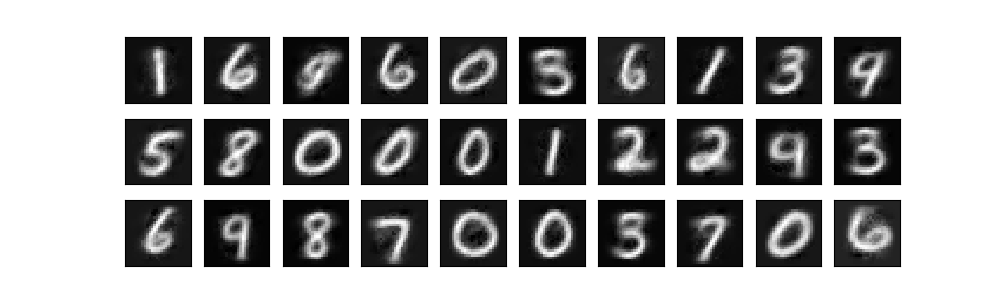
\includegraphics[width=\textwidth]{mnist30_hqkmeans_centroids.png}
\caption{Hierarchical-\palm \qkmeans centroids.}
\label{fig:mnist:hqkmeans:centroids}
\end{subfigure}
\begin{subfigure}[t]{.49\textwidth}
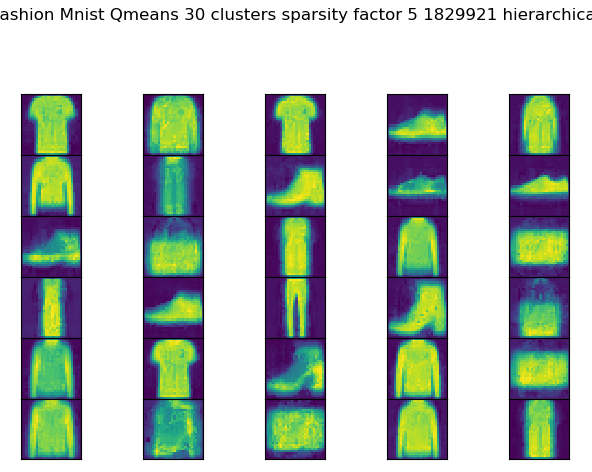
\includegraphics[width=\textwidth]{fashmnist30_hqkmeans_centroids.png}
\caption{Hierarchical-\palm \qkmeans centroids.}
\label{fig:fmnist:hqkmeans:centroids}
\end{subfigure}
\caption{Clustering results on MNIST (left) and Fashion-MNIST (right) for $\nclusters=30$ clusters.}
\label{fig:clustering:realdata}
\end{figure}

\paragraph{Approximation quality.} One important question is the ability of the fast-structure model to fit arbitrary data.
Indeed, no theoretical result about the expressivity of such models is currently available.
In order to assess this approximation quality, the MNIST et Fashion MNIST data have been clustered into $\nclusters=30$ clusters by \kmeans, \qkmeans and a variant of \qkmeans using the hierarchical version of \palm, with several sparsity levels.
Results are reported in Figure~\ref{fig:clustering:realdata}.
In Figures~\ref{fig:mnist:objfun} and~\ref{fig:fmnist:objfun}, one can observe that the objective function of \qkmeans is decreasing in a similar way as \kmeans over iterations.
In particular, the use of the fast-structure model does not seem to slow the procedure down.
At the end of the iterations, the value of objective function for \qkmeans is slightly above that of \kmeans.
As expected, the sparser the model, the more degradation in the objective function.
However, even very sparse models do not degrade the results significantly.
The approximation quality can be assessed visually, in a more subjective and interpretable way, in Figures~\ref{fig:mnist:kmeans:centroids} to~\ref{fig:fmnist:hqkmeans:centroids} where the obtained centroids are displayed as images.
Although some degradation may be observed in some images, one can note that each image obtained with \qkmeans clearly represents a single visual item without noticeable interference with other items.

\paragraph{Clustering assignation times.}
Higher dimensions are required to assess the computational benefits of the proposed approach, as shown here.
The assignation times of the clustering procedure were measured on the Blobs dataset.
The centroid matrices are with shape $\nclusters \times \datadim$ with $\datadim=1000$  and $\nclusters\in\left \lbrace 128, 256, 512\right \rbrace$.
Results reported in Figure~\ref{fig:clustering:blobs:assignation_time} show that in this setting and with the current implementation, the computational advantage of \qkmeans is observed for the higher number of clusters $\nclusters=512$.

%\todo[inline]{Montrer ensuite les temps d'assignation en mode batch 5000 sur blobs, cf. Figure~\ref{fig:clustering:blobs:assignation_time}. Objectif: montrer qu'à partir d'une certaine dimension, \qkmeans est plus rapide.}
%on-line\footnote{Anonymous URL.}.

\begin{figure}[tbh]
\centering
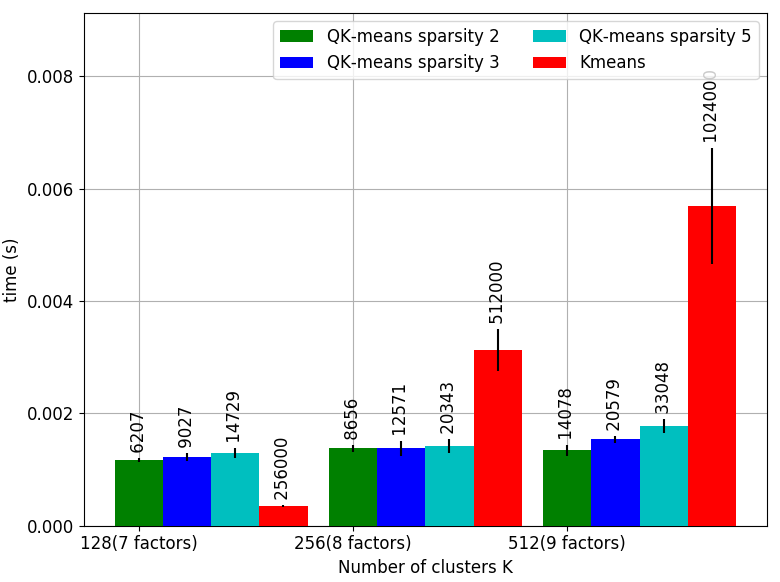
\includegraphics[width=.8\textwidth]{blobs_assignation_time.png}
\caption{Clustering Blobs data: running times of the assignation step, averaged over 5 runs, for batches of $\nexamples=5000$ examples in dimension $\datadim=1000$. The vertical black lines are the standard deviation w.r.t. the runs and the average number of parameters actually learned  in the models are reported above those lines.\addVE{to be completed}.}
\label{fig:clustering:blobs:assignation_time}
\end{figure}

\subsection{Nearest-neighbor search in a large dataset}
Nearest-neighbor search is a fundamental task that suffers from computational limitations when the dataset is large.
Fast strategies have been proposed, e.g., using kd trees or ball trees.
One may also use a clustering strategy to perform an approximate nearest-neighbor search: the query is first compared to $\nclusters$ centroids computed beforehand by clustering the whole dataset, and the nearest neighbor search is then performed among a lower number of data points, within the related cluster.
We compare this strategy using \kmeans and \qkmeans against the \texttt{scikit-learn} implementation~\cite{Pedregosa2011Scikit} of the nearest-neighbor search (naive search, kd tree, ball tree).
Results are reported in Figure~\ref{fig:nn:blobs}.
As shown in Figure~\ref{fig:nn:blobs:accuracy}, the accuracy of the approximate nearest neighbor search is above $0.99$ \todo{Accuracy $>0.99$ to be checked} for all the tested variants of \qkmeans, which is an solid evidence about the reliability of the approach. \addLG{Faire plutôt un grand tableau qui recense tous les résultats d'accuracy sur tous les jeux de données}
The running times reported in Figure~\ref{fig:nn:blobs:times} show a dramatic advantage of using a clustering-based approximate search\todo{to be completed by reporting the actual acceleration ratio obtained by \qkmeans over the three sklearn options.}.

\begin{figure}[tbh]
\centering
\begin{subfigure}[b]{.49\textwidth}
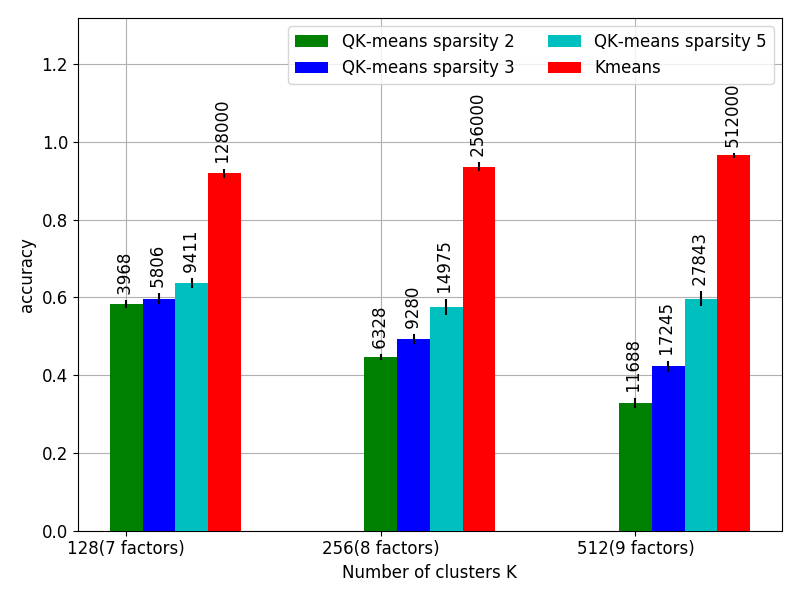
\includegraphics[width=\textwidth]{blobs_1nn_accuracy.png}
\caption{Accuracy.}
\label{fig:nn:blobs:accuracy}
\end{subfigure}
\begin{subfigure}[b]{.49\textwidth}
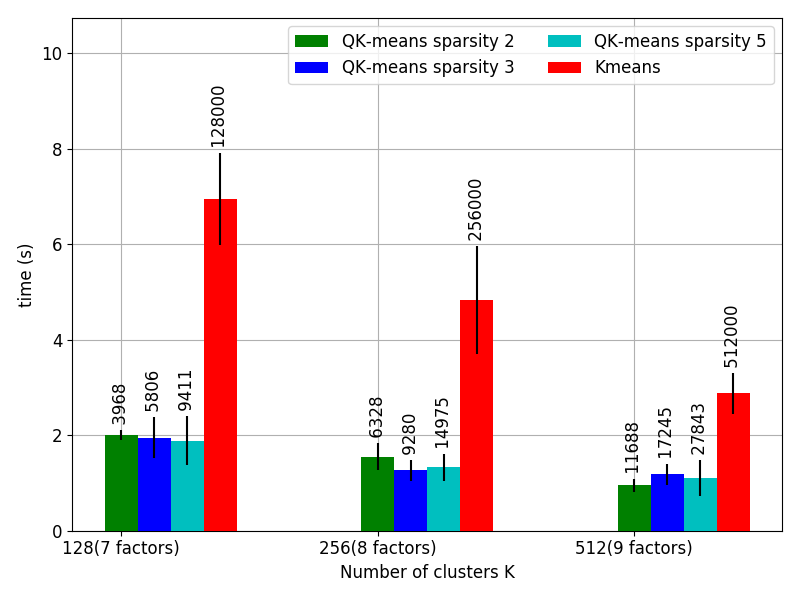
\includegraphics[width=\textwidth]{blobs_1nn_inference_time.png}
\caption{Running times.}
\label{fig:nn:blobs:times}
\end{subfigure}

\caption{Nearest neighbor search on blobs data. Results are averaged over 5 runs (vertical lines: standard deviation) and the average number of parameters actually learned is reported above each bar. \addVE{to be completed: how many runs?}. \addLG{les résultats avec brute/kdtree/balltree ne sont pas affichés car ils prennaient plus de 10 fois le temps de l'approximation avec K means -> peut-être montrer ces résultats de perf avec mnist/fashionmnsit}}
\label{fig:nn:blobs}
\end{figure}

\subsection{Nyström approximation}
\todo[inline]{Sur blobs seulement pour pouvoir être dans des dimensions où \qkmeans est plus rapide. Objectif: montrer la rapidité et une perte limitée de l'accuracy. Se comparer brute/ball tree/KD tree, ce qui donne une grande pertinence car ce sont déjà des approches efficaces. Afficher 2 figures: accuracy et inference time (ou distance time). Figure~\ref{fig:nystrom:blobs}.}

Standard kernel machines are often impossible to use in large-scale applications because of their high computational cost associated with the kernel matrix $\rmK$ which has $O(n^2)$ storage and $O(n^2d)$ computational complexity: $\forall i,j \in\intint{\nexamples}, \rmK_{i,j} = k(\rvx_i, \rvx_j)$. A well-known strategy to overcome this problem is to use the Nyström method which computes a low-rank approximation of the kernel matrix on the basis of some pre-selected landmark points. 

Given $K \ll n$ landmark points $\{\rmU_i\}_{i=1}^{K}$, the Nyström method gives the following approximation of the full kernel matrix:
%
\begin{equation}
 \label{eq:nystrom}
 \rmK \approx \tilde\rmK = \rmC\rmW^\dagger\rmC^T,
\end{equation}
%
with $\rmW \in \R^{K \times K}$ containing all the kernel values between landmarks: $\forall i,j \in [\![K]\!]~ \rmW_{i,j} = k(\rmU_i, \rmU_j)$; $\rmW^\dagger$ being the pseudo-inverse of $\rmW$ and $\rmC \in \R^{n \times K}$ containing the kernel values between landmark points and all data points: $\forall i \in [\![n]\!], \forall j \in [\![K]\!]~ \rmC_{i, j} = k(\rmX_i, \rmU_j)$.

\subsubsection{Efficient Nyström approximation}

A substantial amount of research has been conducted toward landmark point selection methods for improved approximation accuracy \cite{kumar2012sampling} \cite{musco2017recursive}, but much less has been done to improve computation speed. In \cite{si2016computationally}, the authors propose an algorithm to learn the matrix of landmark points with some structure constraint, so that its utilisation is fast, taking advantage of fast-transforms. This results in an efficient Nyström approximation that is faster to use both in the training and testing phases of some ulterior machine learning application.

Remarking that the main computation cost of the Nyström approximation comes from the computation of the kernel function between the train/test samples and the landmark points, \cite{si2016computationally} aim at accelerating this step. In particular, they focus on a family of kernel functions that has the following form:
%
\begin{equation}
 K(\rvx_i, \rvx_j) = f(\rvx_i) f(\rvx_j) g(\rvx_i^T\rvx_j),
\end{equation}
%
where $f: \R^d \rightarrow \R$ and $g: \R \rightarrow \R$. They show that this family of functions contains some widely used kernels such as the Gaussian and the polynomial kernel. Given a set of $K$ landmark points $\rmU \in \R^{K \times d}$ and a sample $\rvx$, the computational time for computing the kernel between $\rvx$ and each row of $\rmU$ (necessary for the Nyström approximation) is bottlenecked by the computation of the product $\rmU\rvx$. They hence propose to write the $\rmU$ matrix as the concatenation of structured $s = K / d$ product of matrices:
%
\begin{equation}
 \rmU = \left[ \rmV_1 \rmH^T, \cdots, \rmV_s\rmH^T  \right]^T,
\end{equation}
%
where the $\rmH$ is a $d \times d$ matrix associated with a fast transform such as the \textit{Haar} or \textit{Hadamard} matrix, and the $\rmV_i$s are some $d \times d$ diagonal matrices to be either chosen with a standard landmark selection method or learned using an algorithm they provide.

Depending on the $\rmH$ matrix chosen, it is possible to improve the time complexity for the computation of $\rmU\rvx$ from $O(Kd)$ to $O(K \log{d})$ (\textit{Fast Hadamard transform}) or $O(K)$ (\textit{Fast Haar Transform}).

\subsubsection{Q-means in Nyström}

We propose to use our Q-means algorithm in order to learn directly the $\rmU$ matrix in the Nyström approximation so that the matrix-vector multiplication $\rmU \rvx$ is cheap to compute, but the structure of $\rmU$ is not constrained by some pre-defined transform matrix. We propose to take the objective $\rmU$ matrix as the K-means matrix of $\rmX$ since it has been shown to achieve good reconstruction accuracy in the Nyström method.


Our algorithm could allow one to obtain an efficient Nyström approximation, while keeping the quality of the K-means landmark points which are expressed as a factorization of sparse matrix.  

\begin{figure}[tbh]
\centering
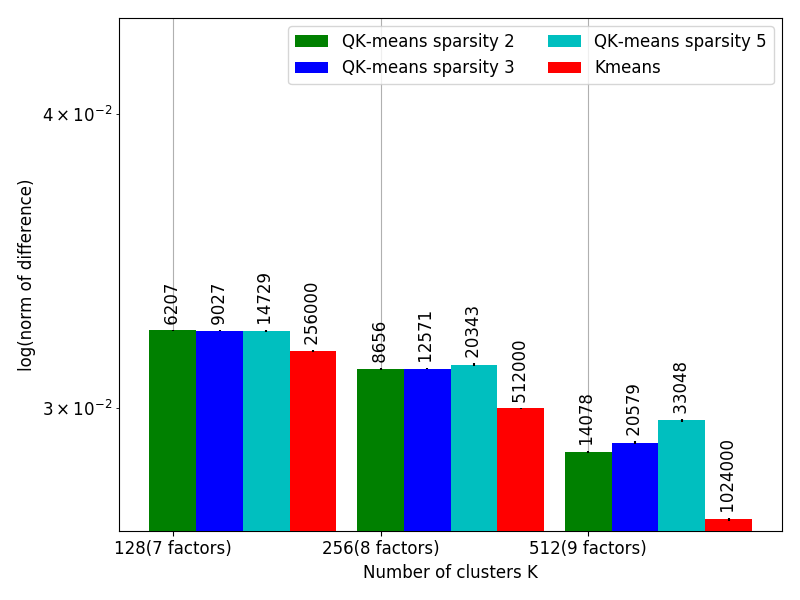
\includegraphics[width=.46\textwidth]{blobs_nystrom_error.png}
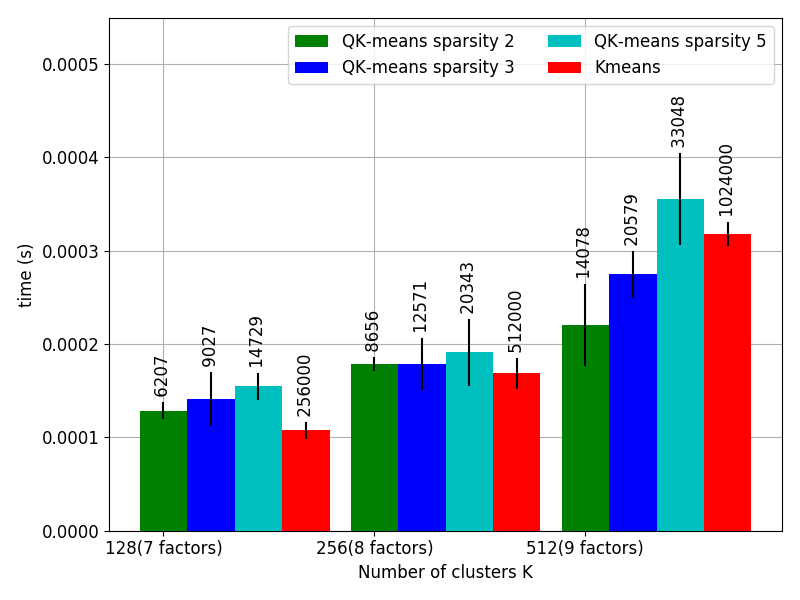
\includegraphics[width=.46\textwidth]{blobs_nystrom_inference_time.png}

\caption{N\"ystrom approximation on blobs data: accuracy (left) and running times (right) \addVE{to be completed}.}
\label{fig:nystrom:blobs}
\end{figure}

%{RBF networks}

%Besoin d'éclaircir les liens avec RBF networks

%\subsection{nearest-neighbours}

%Besoin d'éclaircir les liens avec nearest neighbours
